%% LyX 2.4.4 created this file.  For more info, see https://www.lyx.org/.
%% Do not edit unless you really know what you are doing.
\documentclass[english]{article}
\usepackage[T1]{fontenc}
\usepackage[latin9]{inputenc}
\usepackage{amsmath}
\usepackage{amsthm}
\usepackage{geometry}
\geometry{verbose,tmargin=1in,bmargin=1in,lmargin=1in,rmargin=1in}

\makeatletter
%%%%%%%%%%%%%%%%%%%%%%%%%%%%%% User specified LaTeX commands.
\usepackage{fancyhdr}
\usepackage{lastpage}
\pagestyle{fancy}
\usepackage{enumitem}
\usepackage{tikz}
\usetikzlibrary{shapes,snakes}
\usepackage{amsmath,amssymb}
\usepackage{multicol}
% Added by lyx2lyx
\setlength{\parskip}{\smallskipamount}
\setlength{\parindent}{0pt}

\makeatother

\usepackage{babel}
\begin{document}
\lhead{MTH 331(A) Dr.\,James Ashe}
\chead{\textbf{Helpful Results}}
\cfoot{\thepage{}~of~\pageref{LastPage}}
%%
%%\setenumerate[0]{leftmargin=12pt,itemindent=0pt,labelwidth=0pt}
\renewcommand{\labelenumi}{\textbf{\arabic{enumi}.}}\vspace{-1cm}

\subsection*{13 Functions of Several Variables}

\textbf{Chain Rule (Two Independent Variables). }Let $z$ be a differentiable
function of $x$ and $y,$ where $x$ and $y$ are differentiable
functions of $s$ and $t$. Then 
\[
\frac{dz}{dt}=\frac{dz}{dx}\frac{dx}{dt}+\frac{dz}{dy}\frac{dy}{dt}\mbox{.}
\]
\vfill

\textbf{Gradient (Two Dimensions). }Let $f$ be differentiable at
the point $(x,y)$. The \textbf{gradient} of $f$ at $(x,y)$ is the
vector-valued function 
\[
\nabla f(x,y)=\left\langle f_{x}(x,y),f_{y}(x,y)\right\rangle =f_{x}(x,y)\mathbf{i}+f_{y}(x,y)\mathbf{j}\mbox{.}
\]
\vfill

\textbf{Directional Derivative. }Let $f$ be differentiable at $(a,b)$
and let $\mathbf{u}=\left\langle u_{1},u_{2}\right\rangle $ be a
unit vector in the \emph{xy-}plane, the \textbf{directional derivative
of $f$ at $\left(a,b\right)$ in the direction of u }is 
\[
D_{\mathbf{u}}f(a,b)=\left\langle f_{x}(a,b),f_{y}(a,b)\right\rangle \cdot\left\langle u_{1},u_{2}\right\rangle 
\]

\[
D_{\mathbf{u}}f(a,b)=\nabla f(a,b)\cdot\mathbf{u}\mbox{.}
\]
\vfill

\textbf{Second Derivative Test. }Suppose that the second partial derivatives
of $f$ are continuous throughout an open disk centered at the point
$(a,b)$, where $f_{x}(a,b)=f_{y}(a,b)=0$. Let $D(x,y)=f_{xx}f_{yy}-f_{xy}^{2}$.
\begin{enumerate}
\item If $D(a,b)>0$ and $f_{xx}(a,b)<0$, then $f$ has a local maximum
value at $(a,b)$.
\item If $D(a,b)>0$ and $f_{xx}(a,b)>0$, then $f$ has a local minimum
value at $(a,b)$.
\item If $D(a,b)<0$, then $f$ has a saddle point at $(a,b)$.
\item If $D(a,b)=0$, then the test is inconclusive.\vfill
\end{enumerate}
\begin{multicols}{2}

\subsection*{Helpful formulas}
\begin{enumerate}
\item $\frac{d}{dx}\left(x^{n}\right)=nx^{n-1}$
\item $\frac{d}{dx}\left[f\left(g(x)\right)\right]=f'\left(g(x)\right)\cdot g'(x)$
(Chain rule)
\item $\frac{d}{dx}\left(f(x)g(x)\right)=f'(x)g(x)+f(x)g'(x)$
\item $\frac{d}{dx}e^{x}=e^{x}$
\item $\frac{d}{dx}\sin ax=a\cos ax$
\item $\frac{d}{dx}\cos ax=-a\sin ax$
\item $\int x^{n}\,dx=\frac{1}{n+1}x^{n+1}+C$; $n\neq1$ 
\item $\int\cos ax\,dx=\frac{1}{a}\sin ax+C$
\item $\int\sin ax\,dx=-\frac{1}{a}\cos ax+C$
\item $\int\cos^{2}x\,dx=\frac{x}{2}+\frac{\sin2x}{4}+C$
\item $\int\sin^{2}x\,dx=\frac{x}{2}-\frac{\sin2x}{4}+C$%\vfill
\columnbreak
\end{enumerate}
\footnotesize

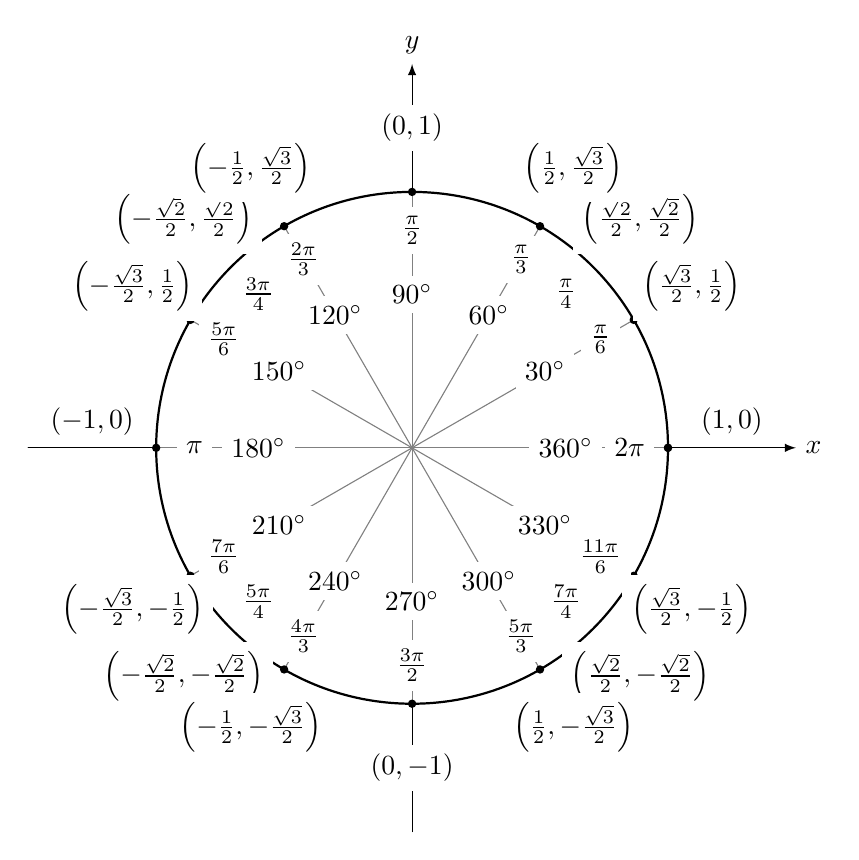
\begin{tikzpicture}[scale=3.25,cap=round,>=latex]         %scale=5,3 % draw the coordinates         
	\draw[->] (-1.5cm,0cm) -- (1.5cm,0cm) node[right,fill=white] {$x$};         
	\draw[->] (0cm,-1.5cm) -- (0cm,1.5cm) node[above,fill=white] {$y$};
        % draw the unit circle         
	\draw[thick] (0cm,0cm) circle(1cm);
    \foreach \x in {0,30,...,360} {                 % lines from center to point                 
			\draw[gray] (0cm,0cm) -- (\x:1cm);                 % dots at each point                 
			\filldraw[black] (\x:1cm) circle(0.4pt);                 % draw each angle in degrees                 
			\draw (\x:0.6cm) node[fill=white] {$\x^\circ$};         
			}
        % draw each angle in radians         
	\foreach \x/\xtext in {
		30/\frac{\pi}{6},             
		45/\frac{\pi}{4},             
		60/\frac{\pi}{3},             			
		90/\frac{\pi}{2},             
		120/\frac{2\pi}{3},             
		135/\frac{3\pi}{4},             
		150/\frac{5\pi}{6},             
		180/\pi,             	
		210/\frac{7\pi}{6},             
		225/\frac{5\pi}{4},             
		240/\frac{4\pi}{3},             
		270/\frac{3\pi}{2},             			
		300/\frac{5\pi}{3},             		
		315/\frac{7\pi}{4},            
		330/\frac{11\pi}{6},             
		360/2\pi}                 
			\draw (\x:0.85cm) node[fill=white] {$\xtext$};
	\foreach \x/\xtext/\y in {             % the coordinates for the first quadrant             
		30/\frac{\sqrt{3}}{2}/\frac{1}{2},             			
		45/\frac{\sqrt{2}}{2}/\frac{\sqrt{2}}{2},             
		60/\frac{1}{2}/\frac{\sqrt{3}}{2},             % the coordinates for the second quadrant             
		150/-\frac{\sqrt{3}}{2}/\frac{1}{2},             
		135/-\frac{\sqrt{2}}{2}/\frac{\sqrt{2}}{2},             			
		120/-\frac{1}{2}/\frac{\sqrt{3}}{2},             % the coordinates for the third quadrant             
		210/-\frac{\sqrt{3}}{2}/-\frac{1}{2},             
		225/-\frac{\sqrt{2}}{2}/-\frac{\sqrt{2}}{2},             
		240/-\frac{1}{2}/-\frac{\sqrt{3}}{2},             % the coordinates for the fourth quadrant             
		330/\frac{\sqrt{3}}{2}/-\frac{1}{2},             				
		315/\frac{\sqrt{2}}{2}/-\frac{\sqrt{2}}{2},             
		300/\frac{1}{2}/-\frac{\sqrt{3}}{2}}                 
			\draw (\x:1.261cm) node[fill=white] {$\left(\xtext,\y\right)$};
        % draw the horizontal and vertical coordinates         % the placement is better this way         
	\draw (-1.25cm,0cm) node[above=1pt] {$(-1,0)$}               
		  (1.25cm,0cm)  node[above=1pt] {$(1,0)$}               
		  (0cm,-1.25cm) node[fill=white] {$(0,-1)$}               
          (0cm,1.25cm)  node[fill=white] {$(0,1)$};     
\end{tikzpicture}

\end{multicols}
\end{document}
